\documentclass[naustrian]{beamer}
\usepackage[T1]{fontenc}
\usepackage[utf8]{inputenc}
\usepackage[ngerman]{babel}
\usetheme{metropolis}           % Use metropolis theme
\title{VIS: OPTICS$_\text{vis}$\\Milestone 3}
\date{\today}
\author{Group 11}
\institute{Fakultät für Informatik}
\titlegraphic{\hfill
\includegraphics[height=1cm]{img/uni_logo_farbe.pdf}}

\definecolor{asparagus}{rgb}{0.53, 0.66, 0.42}
\definecolor{alizarin}{rgb}{0.82, 0.1, 0.26}

\setbeamersize{description width=0.57cm}

\begin{document}
\maketitle

\begin{frame}{Agenda}
    \setbeamertemplate{section in toc}[sections numbered]
    \tableofcontents
\end{frame}

\section{Project}

\subsection{Definition}

\begin{frame}{Project definition}
    \begin{itemize}
        \item OPTICS: density based clustering
            \begin{itemize}
                \item algorithm jumps between points in some order
                \item records jump distances
            \end{itemize}
        \item output somewhat hard to read
            \begin{itemize}
                \item point order
                \item a list of numbers
            \end{itemize}
        \item staple visualization method: the bar chart
    \end{itemize}
    \begin{figure}[h]
        \centering
        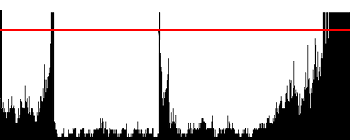
\includegraphics[height=.3\textheight]{img/optics-edited}
        \vspace{1em}
        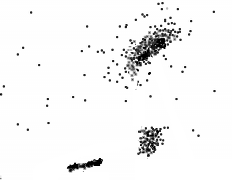
\includegraphics[width=.3\textwidth]{img/optics-edited-points-black}
    \end{figure}
\end{frame}

\begin{frame}{Project definition}
    \begin{itemize}
        \item colorizing helps a lot
        \item but how does it \emph{work}?
        \item how do these numbers relate to the data?
            \begin{itemize}
                \item[] $\rightarrow$ OPTICS$_\text{vis}$
            \end{itemize}
    \end{itemize}
    \begin{figure}[h]
        \centering
        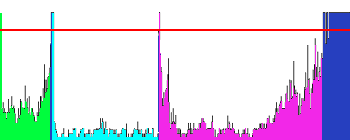
\includegraphics[height=.3\textheight]{img/optics-edited-color}
        \vspace{1em}
        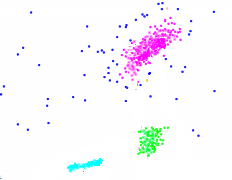
\includegraphics[width=.3\textwidth]{img/optics-edited-points}
    \end{figure}
\end{frame}

\subsection{Data}

\begin{frame}{Our data}
    \begin{itemize}
        \item threefold:
            \begin{enumerate}
                \item points: real-valued and two dimensional (user input)
                \item algorithm output: point ordering and reachability distances
                \item metadata: to be collected as the algorithm runs
            \end{enumerate}
        \item visualize both the data set and the results
        \item give a rough overview of the steps the algorithm did
    \end{itemize}
\end{frame}

\section{Users and Tasks}

\begin{frame}{Users}
\end{frame}

\begin{frame}{Tasks}
\end{frame}

{
\metroset{sectionpage=none}
\section{Demo}
}

\plain{Demo}

\section{Visualization techniques}

\begin{frame}{Visualization techniques}
    \begin{itemize}
        \item filtering
        \item linking \& brushing
        \item tooltips
        \item zooming
        \item heat map
        \item scented widget
        \item aggregation
    \end{itemize}
\end{frame}

\section{Challenges and Problems}

\begin{frame}{Challenges and Problems}
    \begin{itemize}
        \item slow implementation
        \item bla bla
        \item bla
    \end{itemize}
\end{frame}

\end{document}
